\chapter{Présentation de l'interface utilisateur}

    Nous avons choisi une interface en ligne de commande pour ce projet. En effet, nous avons préféré nous investir dans le fond et terminer un maximum de fonctionnalités plutôt que de passer du temps sur une interface graphique dont l'intérêt pour un projet comme celui-là reste limité. L'interface présentée est celle de l'ordonnanceur séquentiel.

    \vfill
    \begin{figure}[!h]
        \centerline {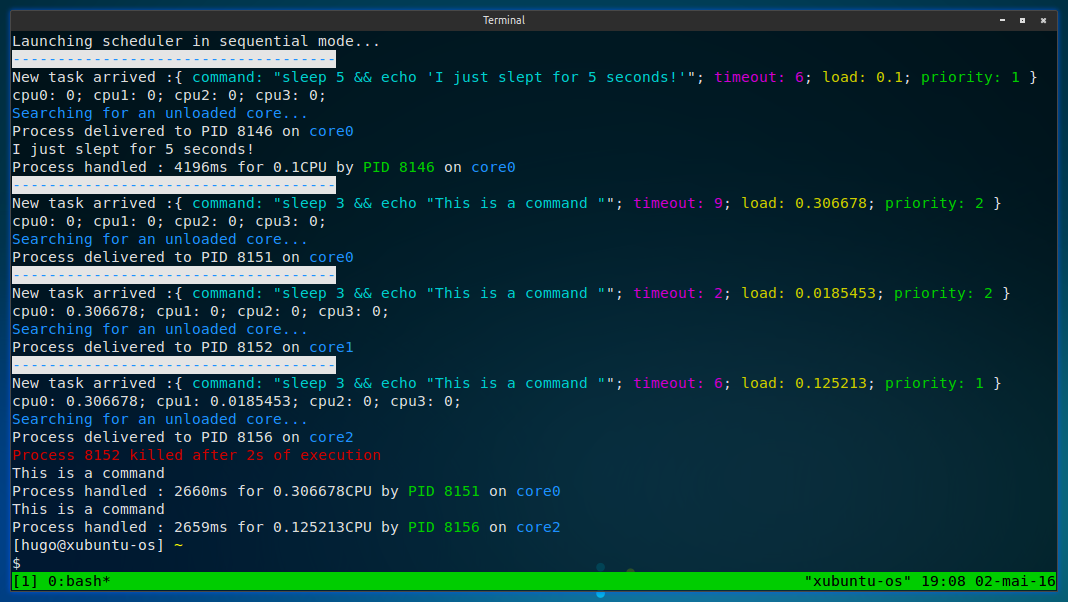
\includegraphics[scale=0.5]{images/scheduler-s.png}}
        \caption{Affichage sheduler du programme}
        \label{Affichage scheduler du programme}
    \end{figure}
    
    \begin{figure}[!t]
        \centering
        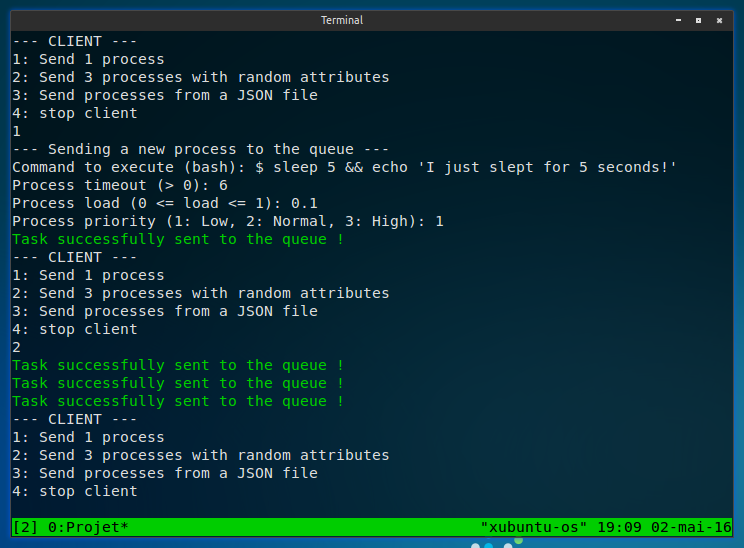
\includegraphics[scale=0.5]{images/scheduler-c.png}
        \caption{Affichage client du programme}
        \label{Affichage client du programme}
    \end{figure}

    Après avoir lancé le scheduler puis le client sur deux émulateurs de terminal différents, l'utilisateur interagit avec le client avec quatre menus principaux :
    
    \begin{itemize}
        \item Send 1 process
        \item Send 3 processes with random attributes
        \item Send processes from a JSON file
        \item Stop client
    \end{itemize}
    
    Il est intéressant de noter que l'ordre de lancement entre les deux programmes importe peu. En revanche, le fait de quitter le client n'arrête pas le scheduler. Lorsque le client est quitté, il faudra attendre que le scheduler s'arrête\footnote{Voir 5.1 Lancement du programme et timeout} (ou l'arrêter de manière brutale). En effet, le canal de communication est ouvert indifféremment pas les deux programmes mais est fermé par le client. Cela est du à une volonté de notre part de pouvoir manipuler le scheduler (démarrage, arrêt, coupure brutale) d'une façon très fluide. \newline
    
    Si l'utilisateur choisit la première option (Send 1 process), alors il lui sera demandé plusieurs attributs à remplir pour que sa tâche soit envoyée au scheduler. Notamment : 
    
    \begin{itemize}
        \item La commande à exécuter (en bash)
        \item Le temps d'expiration (timeout) de la commande (en secondes)
        \item La charge de cette commande sur un processeur (entre 0 et 1)
        \item La priorité de la tâche (entre 1 et 3)
    \end{itemize}
    
    Si la commande à exécuter n'est pas interprétable par un shell, le programme quittera.
    Après avoir remplit tous ces attributs, le client envoie la tâche au scheduler qui la traitera selon notre stratégie d'ordonnancement\footnote{Voir Chapitre 4 Stratégie d’ordonnancement} puis imprime le message suivant à l'écran : "Task successfully sent to the queue !". 
    
    Si l'utilisateur choisit la seconde option (Send 3 processes with random attributes), le client va afficher les tâches qu'il va envoyer au scheduler : "created : { command: "sleep 3 \&\& echo "This is a command ""; timeout: 2; load: 0.627926; priority: 2 }", les envoie au scheduler puis affiche le message suivant : "Task successfully sent to the queue !".
    
    Les résultats seront alors visibles sur l'écran du scheduler qui affiche son traitement comme suit, pour chaque tâche arrivée :
    
    \vbox{
    \begin{verbatim}
------------------------------------
New task arrived :{ command: "sleep 3 && echo "This is a command"";
    timeout: 10; load: 0.960486; priority: 1}
cpu0: 0; cpu1: 0; cpu2: 0; cpu3: 0;
Searching for an unloaded core...
Process delivered to PID 10359 on core0
This is a command // Ici la commande est exécutée.
Process handled : 3010ms for 0.960486CPU by PID 10359 on core0
    \end{verbatim}
    }
    
    En outre, le client peut charger un fichier JSON à partir de la troisième option. Il lui faudra juste préciser le chemin ainsi que le nom du fichier à partir du dossier d'exécution du programme.
    
    Si tout le fichier est écrit correctement alors les messages suivant s'afficheront après la demande du fichier. Si une tâche ne possède pas la bonne syntaxe, la lecture de fichier s'arrêtera et affichera une erreur. 
    
    \vbox{
    \begin{verbatim}
--- Enter the path of json file  ---
test.json
Task successfully sent to the queue !
Task successfully sent to the queue !
....
Task cannot be created. Verify your json file.
    \end{verbatim}
    }

Voici un template de fichier JSON que notre programme pourra analyser. Si jamais il manque un argument(command,timeout,load,priority) le programme entrera lui même l'argument manquant. Cela ne produira pas d'erreur et sera totalement transparent. 

    \vbox{
    \begin{minted}{json}
{
  "0" :{
    "command":"sleep 3 && echo \"This is a command\"",
    "timeout":10,
    "priority":3
  },
  "1":{
    "command":"sleep 3 && echo \"This is a command\"",
    "load":0.5,
    "priority":1
  },
  "2" :{
    "command":"sleep 3 && echo \"This is a command\"",
    "timeout":1,
    "load":0.7,
    "priority":2
  },
  "3" :{
    "command":"sleep 3 && echo \"This is a command\""
  },
  "4" :{
    "command":"sleep 3 && echo \"This is a command\"",
    "timeout":2,
    "load":0.98,
    "priority":3
  }
}
    \end{minted}    
    }
    
    Le scheduler peut aussi afficher d'autres messages différents, mis dans le désordre ici, qui seront détaillés plus tard :
    
    \vbox{
    \begin{verbatim}
...
Process 10359 killed after 2s of execution // Voir 4.4.2 Expiration d’une tâche
...
No unloaded core found ! // Voir 4.1 Algorithme 
Searching for a core that can fit the task...
...
    \end{verbatim}
    }